\documentclass[11pt]{article}

\usepackage[margin=1in]{geometry}
\usepackage{amsmath,amssymb}
\usepackage{booktabs}
\usepackage{longtable}
\usepackage{array}
\usepackage{xcolor}
\usepackage{verbatim}
\usepackage{tikz}
\usepackage{hyperref}
\usetikzlibrary{arrows.meta,positioning,shapes.geometric,fit,calc}

\hypersetup{
  colorlinks=true,
  linkcolor=blue!50!black,
  citecolor=blue!50!black,
  urlcolor=blue!50!black
}

\newcounter{algorithm}
\newcommand{\AlgorithmCaption}[2]{%
  \refstepcounter{algorithm}%
  \label{#1}%
  \par\medskip\noindent\textbf{Algorithm~\thealgorithm. #2}\par\nobreak\smallskip%
}

\newcommand{\clight}{c}
\newcommand{\arad}{a_{\rm r}}
\newcommand{\sigP}{\sigma_{\rm P}}
\newcommand{\sigA}{\sigma_{\rm a}}
\newcommand{\sigS}{\sigma_{\rm s}}
\newcommand{\sigT}{\sigma_{\rm t}}
\newcommand{\dt}{\Delta t}
\newcommand{\dd}{\mathrm{d}}
\newcommand{\Erad}{E_{\rm r}}
\newcommand{\Eg}{E_g}
\newcommand{\vcell}{\mathbf{v}}
\newcommand{\x}{\mathbf{x}}
\newcommand{\mom}{\mathbf{p}}
\newcommand{\OmegaVec}{\boldsymbol{\Omega}}

\title{An Implicit Monte Carlo Radiation Transport Implementation on a Three-Dimensional Voronoi Mesh}
\author{Prepared from the \texttt{RadiationIMC} implementation}
\date{\today}

\begin{document}
\maketitle

\begin{abstract}
This document describes the numerical design implemented in
\texttt{source/3D/radiation/RadiationIMC.cpp} and its associated helper
classes. The implementation is an implicit Monte Carlo (IMC) method for
thermal radiation transport on a three-dimensional Voronoi tessellation. The
method advances weighted photon packets through cell-face crossings, effective
scattering events, and time-census events. Absorption is treated continuously
along each packet trajectory by exponential weight attenuation, with the
absorbed packet energy deposited into the material conserved variables. Thermal
emission over a time step is represented by newly sampled packets whose total
energy is determined by the Fleck linearization. The code also includes
optional hydrodynamic feedback, a lab/comoving-frame Doppler treatment,
multigroup frequency sampling, group-resolved radiation energy tallies,
diffusion-pressure-gradient momentum coupling, an optional moving-material
correction mode, and an implicit random-walk acceleration for optically thick
cells. The emphasis here is not a generic description of IMC, but a detailed
record of the actual numerical algorithm, state variables, event logic, and
approximations embodied in the current implementation.
\end{abstract}

\section{Purpose and Scope}

The IMC module is embedded in a larger Monte Carlo transport framework. The
framework owns particle storage, cell migration, boundary interaction, and MPI
exchange, while \texttt{RadiationIMC} supplies the physics-specific operations:
pre-step source creation, one-particle transport, and post-step material and
radiation updates. The core implementation appears in
\texttt{RadiationIMC.cpp}; multigroup thermal sampling is factored into
\texttt{MultigroupOpacity}; random-walk acceleration is implemented in
\texttt{RadiationIMC\_RandomWalk.cpp} and \texttt{RandomWalk.cpp}; Lorentz and
Doppler operations are implemented in \texttt{LorentzTransformation.cpp}.

The algorithm is designed for radiation hydrodynamics calculations in which
the gas state is represented by \texttt{ComputationalCell3D} objects and
conserved extensive quantities are represented by \texttt{Conserved3D}. Packet
weights are extensive energies. Cell radiation fields stored in the hydro
state, such as \texttt{cell.Erad} and \texttt{cell.Eg[g]}, are specific
radiation energies after normalization by cell mass. During the Monte Carlo
step the packet ensemble carries the extensive radiation energy; at the end of
the step the code reconstructs cell radiation energies by summing packet
weights in each cell.

The implementation should be understood as a mixed exact/stochastic update.
Particle free paths, angular directions, emission points, and thermal
frequencies are sampled. Absorption along a realized path segment is integrated
analytically. The material temperature and pressure are then recovered from the
equation of state after all packet-material energy exchange has been accumulated.

\section{State Variables and Interfaces}

Each Monte Carlo packet is an instance of
\texttt{MonteCarloParticle<Vector3D,Tessellation3D>}. The fields used by the
IMC method are listed in Table~\ref{tab:packet-state}. The packet velocity is a
vector of magnitude \(c\), so the direction is
\(\OmegaVec=\mathbf{u}/c\). The field named \texttt{frequency} is used as the
spectral coordinate passed to the opacity model and compared with
\texttt{ComputationalCell3D::energyBoundaries}; in this implementation it is
therefore best read as a photon energy-like group coordinate.

\begin{table}[htbp]
\centering
\caption{Packet state used by the IMC transport kernel.}
\label{tab:packet-state}
\begin{tabular}{>{\ttfamily}p{0.23\linewidth}p{0.67\linewidth}}
\toprule
Field & Numerical role \\
\midrule
location & Current packet position \(\x\) inside a Voronoi cell. \\
velocity & Transport velocity \(\mathbf{u}=c\OmegaVec\). It is resampled at scattering and after random-walk events. \\
cellIndex & Local index of the Voronoi cell containing the packet. \\
cellID & Persistent cell identifier, used when initial particles are generated. \\
timeLeft & Remaining time to the end-of-step census. \\
frequency & Spectral coordinate used for multigroup opacity and thermal re-emission sampling. \\
weight & Current packet energy weight. Absorption decreases it continuously. \\
initialWeight & Initial packet energy weight, used for Russian-roulette-like removal thresholds. \\
steps & Counter used by the Monte Carlo managers for diagnostics/tracking. \\
\bottomrule
\end{tabular}
\end{table}

The constructor receives references to the tessellation, boundary condition,
cell state, conserved variables, equation of state, opacity calculator, and a
\texttt{RadiationIMCParameters} object. The parameter object selects the
optional physical and numerical branches summarized in
Table~\ref{tab:parameters}. These switches are deliberately orthogonal where
possible: for example, multigroup opacity can be combined with hydrodynamic
feedback and with random-walk acceleration.

\begin{table}[htbp]
\centering
\caption{Main IMC control parameters.}
\label{tab:parameters}
\begin{tabular}{>{\ttfamily}p{0.27\linewidth}p{0.63\linewidth}}
\toprule
Parameter & Effect in the implemented algorithm \\
\midrule
newPhotonsPerCell & Minimum number of newly emitted packets per cell per time step. The actual number is energy-weighted and clamped. \\
withHydro & Enables momentum/energy coupling to the hydrodynamic conserved variables and Doppler/Lorentz transformations when \texttt{MMC} is false. \\
diffusionPressureGradient & Replaces eventwise radiation momentum deposition by a post-step diffusion pressure force based on \(\nabla \langle E_{\rm r}\rangle_t/3\). \\
MMC & Activates the existing-particle moving-material correction in \texttt{adjustExistingParticles}; in this mode the normal per-event Doppler branch is bypassed. \\
withMultigroupOpacity & Uses frequency-dependent absorption opacity and thermal group sampling through \texttt{MultigroupOpacity}. \\
withRandomWalk & Enables implicit random-walk acceleration in optically thick cells. \\
rwMinCellOpticalDepth & Cell-level optical-depth threshold for random-walk eligibility. \\
rwMinParticleOpticalDepth & Particle-centered optical-depth threshold for actually taking a random-walk step. \\
noHydroFeedback & Keeps the transport and radiation tallies active but disables material energy and momentum feedback. \\
withEgTimeAvg & Accumulates group-resolved time-averaged radiation energy when multigroup opacity is enabled. \\
\bottomrule
\end{tabular}
\end{table}

\section{Continuous Equations and IMC Linearization}

The code represents gray or multigroup thermal radiation interacting with a
material through absorption, re-emission, and scattering. In a gray notation,
the radiation-material energy exchange contains the familiar thermal source
and sink terms
\begin{equation}
  \frac{\partial E_{\rm r}}{\partial t}
  + \OmegaVec\cdot\nabla(c E_{\rm r})
  =
  \sigA c\, a_{\rm r}T^4
  - \sigA c\, E_{\rm r}
  + \hbox{scattering terms},
\end{equation}
with a corresponding material internal-energy update. IMC stabilizes the
emission/absorption coupling by linearizing the thermal emission over the full
time step and replacing part of absorption/re-emission by effective scattering.
For each cell \(i\), the implementation computes a Fleck factor
\begin{equation}
  f_i =
  \left[
    1 +
    \frac{4 \arad T_i^3 \sigma_{{\rm P},i} \clight \dt \gamma_i}{c_{v,i}}
  \right]^{-1}.
  \label{eq:fleck}
\end{equation}
Here \(\sigma_{{\rm P},i}\) is \texttt{CalcPlanckOpacity(cell)}, \(c_{v,i}\) is obtained
from \texttt{eos->dT2cv}, and
\begin{equation}
  \gamma_i =
  \begin{cases}
    \left(1-|\vcell_i|^2/c^2\right)^{-1/2}, & \texttt{withHydro} \wedge \neg\texttt{MMC},\\
    1, & \text{otherwise}.
  \end{cases}
\end{equation}
Equation~\eqref{eq:fleck} is the central implicitness mechanism. When the
material-radiation coupling over a step is weak, \(f_i\approx 1\) and the
scheme behaves close to explicit absorption and emission. When the coupling is
stiff, \(f_i\ll 1\) and most would-be absorption/re-emission is converted to
effective scattering, reducing thermal instability without forcing a tiny time
step.

The linearization divides absorption into two pieces:
\begin{equation}
  \sigA
  =
  f_i\sigA + (1-f_i)\sigA .
\end{equation}
The first term is true absorption into the material and is treated by
continuous weight attenuation. The second term is sampled together with
physical scattering as an event opacity
\begin{equation}
  \sigma_{{\rm eff},i}(\epsilon)
  =
  \sigma_{{\rm s},i} + (1-f_i)\sigma_{{\rm a},i}(\epsilon),
  \label{eq:effective-scattering}
\end{equation}
where the energy argument \(\epsilon\) is present in the multigroup branch. At
such an event, the packet direction is resampled. In the multigroup branch the
code then decides whether the event was physical scattering or effective
absorption/re-emission; in the latter case the packet spectral coordinate is
resampled from the cell thermal spectrum.

\section{Time-Step Orchestration}

At the level of \texttt{RadiationMCStep}, each radiation step proceeds through
three physics calls:
\begin{enumerate}
\item Existing particles are optionally updated for hydrodynamic cell motion or
the \texttt{MMC} correction.
\item The Monte Carlo manager calls \texttt{preStep(dt)}, transports all
packets by repeated calls to \texttt{step(particle)}, and applies boundary/cell
movement logic.
\item The manager calls \texttt{postStep(particles,dt)} to normalize tallies,
update material thermodynamics, and rebuild cell radiation energies from the
surviving packet ensemble.
\end{enumerate}

The manager interprets the status returned by the physics kernel as listed in
Table~\ref{tab:events}. A \texttt{CELL\_MOVE} status does not itself mutate the
cell index inside \texttt{RadiationIMC::step}; it asks the manager to either
move the packet to a neighboring cell or apply the boundary condition. This
separation keeps geometry/boundary ownership in the generic transport manager.

\begin{table}[htbp]
\centering
\caption{Particle-status values returned by the physics step.}
\label{tab:events}
\begin{tabular}{>{\ttfamily}p{0.25\linewidth}p{0.65\linewidth}}
\toprule
Status & Meaning in the IMC algorithm \\
\midrule
NO\_CELL\_MOVE & Continue transporting the packet in the same cell. This is also the implicit return after most scatter and random-walk leak/upscatter events. \\
CELL\_MOVE & The packet reached a Voronoi face; the manager changes cells or applies a boundary condition. \\
DONE & The packet reached census, i.e. \texttt{timeLeft} reached zero, and is retained for the next step. \\
REMOVE & The packet has negligible remaining weight or left through an absorbing boundary; the manager deletes it. \\
REFLECT & Boundary-condition return value used by the manager, not directly returned by the IMC physics step. \\
\bottomrule
\end{tabular}
\end{table}

\begin{figure}[htbp]
\centering
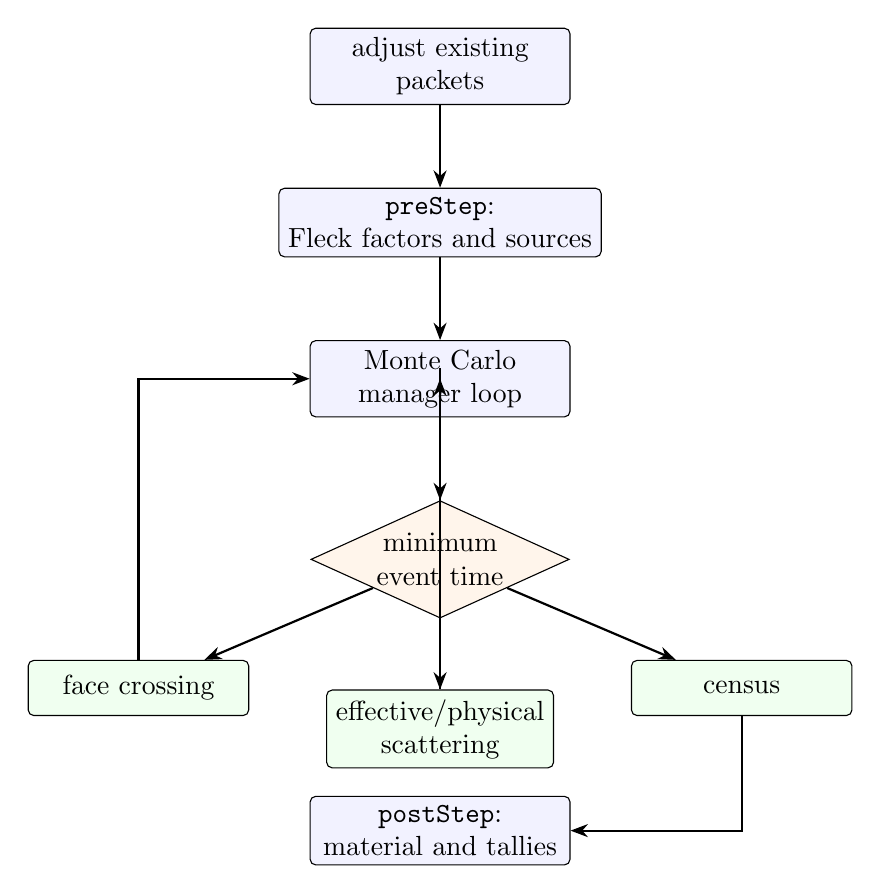
\begin{tikzpicture}[
  node distance=1.05cm,
  box/.style={draw,rounded corners=2pt,align=center,minimum width=3.3cm,minimum height=0.8cm,fill=blue!5},
  smallbox/.style={draw,rounded corners=2pt,align=center,minimum width=2.8cm,minimum height=0.7cm,fill=green!6},
  decision/.style={draw,diamond,aspect=2.2,align=center,inner sep=1pt,fill=orange!8},
  arr/.style={-{Stealth[length=2.2mm]},thick}
]
\node[box] (adjust) {adjust existing\\packets};
\node[box,below=of adjust] (pre) {\texttt{preStep}:\\Fleck factors and sources};
\node[box,below=of pre] (manager) {Monte Carlo\\manager loop};
\node[decision,below=of manager] (event) {minimum\\event time};
\node[smallbox,below left=0.9cm and 1.6cm of event] (face) {face crossing};
\node[smallbox,below=0.9cm of event] (scatter) {effective/physical\\scattering};
\node[smallbox,below right=0.9cm and 1.6cm of event] (census) {census};
\node[box,below=2.25cm of event] (post) {\texttt{postStep}:\\material and tallies};
\draw[arr] (adjust) -- (pre);
\draw[arr] (pre) -- (manager);
\draw[arr] (manager) -- (event);
\draw[arr] (event) -- (face);
\draw[arr] (event) -- (scatter);
\draw[arr] (event) -- (census);
\draw[arr] (face) |- (manager);
\draw[arr] (scatter) |- (manager);
\draw[arr] (census) |- (post);
\end{tikzpicture}
\caption{High-level control flow. The IMC physics module chooses local
transport events; the generic Monte Carlo manager owns repeated stepping,
cell migration, removal, census storage, and boundary-condition application.}
\label{fig:workflow}
\end{figure}

\AlgorithmCaption{alg:macro}{Macro-level radiation time step.}
\begin{verbatim}
procedure RadiationStep(dt):
  if withHydro:
    update particle cell indices on the current tessellation

  adjustExistingParticles(particles, dt)

  newParticles = RadiationIMC.preStep(dt)
  add newParticles to the manager

  for each active packet p:
    while p is active:
      status = RadiationIMC.step(p)
      if status == CELL_MOVE:
        move p to neighbor or apply boundary condition
      else if status == DONE:
        store p as a census particle
        break
      else if status == REMOVE:
        delete p
        break
      else:
        continue in the same cell

  RadiationIMC.postStep(censusParticles, dt)
  suggest next dt from the maximum relative temperature/radiation change
end procedure
\end{verbatim}

\section{Pre-Step: Fleck Factors, Opacities, and Source Packets}

The pre-step stage initializes all quantities that are constant over the
radiation time step. For each cell the code computes the Planck opacity
\(\sigma_{{\rm P},i}\), the Fleck factor \(f_i\), and zeroes the time-averaged radiation
energy arrays. If multigroup opacity is active, the cached cumulative thermal
opacity table is invalidated so that each cell can rebuild it with the current
temperature. If random walk is active, cell eligibility and diffusion
coefficients are also precomputed after the Fleck factors and Planck opacities
are known.

\AlgorithmCaption{alg:prestep}{Pre-step preparation and source generation.}
\begin{verbatim}
procedure preStep(dt):
  for each cell i:
    sigmaP[i] = opacity.CalcPlanckOpacity(cell[i])
    gamma[i] = Lorentz factor if hydro is active and MMC is false, else 1
    cv       = eos.dT2cv(rho[i], T[i], tracers[i])
    f[i]    = 1 / (1 + 4 * arad * T[i]^3 * sigmaP[i] * c * dt * gamma[i] / cv)
    require 0 <= f[i] <= 1
    Erad_time_avg[i] = 0
    Eg_time_avg[i,g] = 0 if requested

  if random walk is active:
    precomputeRandomWalkData()

  emitted = generateParticles(dt)
  boundary = boundary.generateNewBoundaryParticles(dt)
  return emitted plus boundary
end procedure
\end{verbatim}

\subsection{Thermal Emission Energy}

The energy emitted from cell \(i\) during the step is
\begin{equation}
  E^{\rm src}_i
  =
  f_i\,V_i\,\arad T_i^4\,\sigma_{{\rm P},i}\,\clight\,\dt,
  \label{eq:source-energy}
\end{equation}
where \(V_i\) is the cell volume. This energy is immediately subtracted from
the material internal-energy conserved variable unless \texttt{noHydroFeedback}
is active. If hydrodynamic feedback is enabled, the total conserved gas energy
is reduced by \(\gamma_i E^{\rm src}_i\), and, when eventwise momentum coupling
is used, the gas momentum is reduced by
\begin{equation}
  \Delta \mom_i^{\rm src}
  =
  -\gamma_i E^{\rm src}_i\,\frac{\vcell_i}{c^2}.
\end{equation}
This source bookkeeping makes emission conservative at the packet-material
interface: the energy assigned to newly created packets is removed from the
material before transport begins.

\subsection{Packet Number Allocation}

The implementation uses a global emission-energy weighting to distribute
packet counts. First each rank computes its local \(E^{\rm src}_i\), then MPI
reductions obtain the global emitted energy and global cell count. The nominal
global number of source packets is
\begin{equation}
  N_{\rm src}^{\rm target}
  =
  10\,N_{\rm cell}^{\rm global}\,N_{\rm new},
\end{equation}
where \(N_{\rm new}\) is \texttt{newPhotonsPerCell}. The number emitted by
cell \(i\) is then
\begin{equation}
  N_i =
  \max\left[
    N_{\rm new},
    \min\left(
      \left\lfloor
      \frac{E^{\rm src}_i}{E^{\rm src}_{\rm global}}
      N_{\rm src}^{\rm target}
      \right\rfloor,
      20N_{\rm new}
    \right)
  \right].
  \label{eq:packet-count}
\end{equation}
If the global emitted energy is zero, the fallback is \(N_i=N_{\rm new}\).
Thus every cell emits at least a minimum number of packets, but extremely
bright cells are capped to avoid a single cell dominating memory and runtime.

\subsection{Spatial, Angular, and Spectral Sampling}

Each emitted packet is placed at a random point in its Voronoi cell using
\texttt{RandomPointInCell}. The implementation verifies that the point lies in
the selected cell and then nudges it by \(10^{-10}\) of the distance toward the
cell mesh point. This small inward displacement reduces numerical ambiguity for
particles born exactly on a face. The packet direction is isotropic by default:
\texttt{OpacityCalculator::getRandomVelocity} samples a random vector and
normalizes it to speed \(c\). More specialized opacity models can override the
direction or post-scatter angular sampling.

In gray mode, emitted packets have no meaningful spectral coordinate and the
weight is simply the source energy divided by the packet count, modified by the
hydrodynamic Doppler factor if appropriate. In multigroup mode, thermal
emission uses \texttt{MultigroupOpacity::GetThermalEnergy}. For a cell at
temperature \(T\), the helper forms a cumulative array
\begin{equation}
  C_g =
  \sum_{k=1}^{g}
  \sigA(\epsilon_{k-1/2})
  \int_{\epsilon_{k-1}/k_{\rm B}T}^{\epsilon_k/k_{\rm B}T}
  B(x)\,\dd x ,
  \qquad C_0=0,
  \label{eq:opacity-weighted-thermal-cdf}
\end{equation}
where \(\epsilon_g\) are group boundaries and \(\epsilon_{k-1/2}\) are group
centers. A uniform random number \(\xi\) selects an energy by linear
interpolation in \(C_g\) at \(\xi C_{G}\). This is an opacity-weighted thermal
emissivity distribution, not merely a Planck distribution. Initial particles,
by contrast, are sampled from a pure Planck cumulative distribution because
they represent an already existing radiation energy density rather than new
material emission.

\subsection{Moving Materials and Packet Weights}

When \texttt{withHydro} is true and \texttt{MMC} is false, packet directions
are sampled in the comoving frame and then transformed to the lab frame by
\texttt{LorentzTransformation(particle, -cell.velocity)}. The Doppler factor
used throughout the implementation is
\begin{equation}
  D(\mathbf{u},\vcell)
  =
  \gamma\left(1-\frac{\vcell\cdot\mathbf{u}}{c^2}\right),
  \label{eq:doppler}
\end{equation}
where \(\mathbf{u}\) is the packet velocity vector. Source-packet lab-frame
weights are initialized as \(E^{\rm src}_i/(N_iD)\), and multigroup source
frequencies are sampled in the comoving frame and divided by \(D\) to obtain
the lab-frame spectral coordinate. This convention is consistent with the
later transport step, where the code multiplies the lab-frame spectral
coordinate by \(D\) before evaluating frequency-dependent absorption opacity.

\section{Single-Packet Transport Kernel}

The method \texttt{RadiationIMC::step} advances one packet until the next of
three competing events occurs:
\begin{equation}
  \delta t
  =
  \min
  \left(
    t_{\rm face},
    t_{\rm sca},
    t_{\rm census}
  \right).
  \label{eq:event-min}
\end{equation}
Here \(t_{\rm face}\) is the time to the next Voronoi face, computed by the
base Monte Carlo geometry routines; \(t_{\rm census}\) is the packet
\texttt{timeLeft}; and \(t_{\rm sca}\) is sampled from the effective scattering
opacity. Before the analog event competition, the code may attempt a
random-walk step if the current cell and particle are optically thick enough.
If the random-walk step succeeds, \texttt{step} returns immediately.

\AlgorithmCaption{alg:packet-step}{Core analog IMC packet step.}
\begin{verbatim}
procedure step(packet p):
  i = p.cellIndex
  (face, tFace, nextCell) = getIntersectionDetails(p)
  D = DopplerShift(p, cell[i].velocity) if hydro and not MMC, else 1

  if randomWalk is enabled and cell i is eligible:
    if tryRandomWalkStep(p, D) succeeds:
      return status produced by random walk

  if multigroup:
    epsCo = clamp(p.frequency * D)
    sigmaA = opacity.CalcAbsorptionOpacity(cell[i], epsCo)
  else:
    sigmaA = planckOpacity[i]

  sigmaS = opacity.CalcScatteringOpacity(cell[i])
  sigmaEvent = sigmaS + (1 - f[i]) * sigmaA
  tScatter = -log(1 - xi) / (D * c * sigmaEvent)

  dtLocal = min(tFace, tScatter, p.timeLeft)
  p.timeLeft -= dtLocal

  // Continuous true absorption over the segment.
  rateCo = sigmaA * f[i] * c
  attenLab = exp(-D * rateCo * dtLocal)
  attenCo  = exp(-rateCo * dtLocal)
  deposit material energy proportional to (1 - attenCo)
  deposit material momentum proportional to (1 - attenLab) if requested
  accumulate time-averaged radiation energy
  p.weight *= attenLab
  p.location += p.velocity * dtLocal

  if p.weight is below 1e-3 of p.initialWeight:
    deposit residual weight and return REMOVE

  if dtLocal == tFace:
    return CELL_MOVE with nextCell
  else if dtLocal == tScatter:
    process scatter/effective-scatter event
    return NO_CELL_MOVE
  else:
    return DONE
end procedure
\end{verbatim}

\subsection{Effective Scattering Distance}

The sampled interaction length is
\begin{equation}
  \ell_{\rm sca}
  =
  \frac{-\ln(1-\xi)}
       {D\,[\sigma_{{\rm s},i}+(1-f_i)\sigma_{{\rm a},i}]},
  \qquad
  t_{\rm sca}=\frac{\ell_{\rm sca}}{|\mathbf{u}|}.
  \label{eq:scattering-distance}
\end{equation}
Since \(|\mathbf{u}|=c\), this is equivalent to sampling an event time from
rate \(D c[\sigma_{{\rm s},i}+(1-f_i)\sigma_{{\rm a},i}]\). The Doppler factor is one unless the
hydrodynamic moving-medium branch is active. The code explicitly checks for
negative sampled distances and negative local time steps, attaching diagnostic
entries such as opacity, Fleck factor, Doppler shift, and packet state to a
\texttt{UniversalError}.

\subsection{Continuous Absorption and Time Averages}

Along the selected path segment of duration \(\delta t\), true absorption is
integrated analytically rather than sampled as a discrete event. Define
\begin{equation}
  r_i = f_i\sigma_{{\rm a},i} c.
\end{equation}
The packet weight is attenuated by the lab-frame factor
\begin{equation}
  w^{n+1} = w^n\exp(-D r_i\delta t),
  \label{eq:weight-attenuation}
\end{equation}
while the material internal-energy conserved variable receives
\begin{equation}
  \Delta E_{{\rm mat},i}
  =
  w^n\left[1-\exp(-r_i\delta t)\right],
  \label{eq:material-deposit}
\end{equation}
when feedback is enabled. The distinction between
Equations~\eqref{eq:weight-attenuation} and \eqref{eq:material-deposit} is
intentional in the code: the packet's transported lab energy follows the
Doppler-shifted attenuation, whereas the material heating tally uses the
comoving absorption rate. When hydrodynamic momentum feedback is eventwise
rather than pressure-gradient based, the code adds
\begin{equation}
  \Delta \mom_{{\rm mat},i}
  =
  w^n\left[1-\exp(-D r_i\delta t)\right]
  \frac{\mathbf{u}}{c^2}.
  \label{eq:momentum-deposit}
\end{equation}

The same exponential solution is used to tally time-averaged radiation energy.
For each segment the unnormalized contribution is
\begin{equation}
  \int_0^{\delta t} w^n\exp(-r_i t)\,\dd t
  =
  w^n\frac{1-\exp(-r_i\delta t)}{r_i}.
  \label{eq:time-average-segment}
\end{equation}
The implementation accumulates this quantity as
\texttt{Erad\_time\_avg[i]} and, if requested, also as
\texttt{Eg\_time\_avg[i][g]} for the packet's energy group. Post-step
normalization divides by \(V_i\dt\), producing a time-averaged radiation energy
density. This time-centered quantity is later used by the optional
diffusion-pressure-gradient force.

\subsection{Low-Weight Removal}

After absorption, if the packet weight has fallen below \(10^{-3}\) of
\texttt{initialWeight}, the packet is removed. Its remaining weight is deposited
into the material internal energy when feedback is active. This deterministic
cutoff prevents packets with negligible contribution from consuming transport
cycles indefinitely. The random-walk branch uses an even smaller threshold,
\(10^{-4}\), because a random-walk step may already represent many physical
collisions.

\section{Scattering, Effective Re-Emission, and Multigroup Updates}

If the sampled event is scattering, the packet direction is first updated by
\texttt{opacity->getNewScatterVelocity}. The default opacity implementation
resamples an isotropic direction, but the virtual interface allows anisotropic
or frequency-changing scattering laws to be inserted.

In multigroup mode the packet spectral coordinate is then converted from lab to
comoving by multiplication with the Doppler factor and clamped to the global
energy bounds. The event is classified as effective re-emission with
probability
\begin{equation}
  P_{\rm eff}
  =
  \frac{(1-f_i)\sigma_{{\rm a},i}}
       {(1-f_i)\sigma_{{\rm a},i}+\sigma_{{\rm s},i}}.
  \label{eq:effective-scattering-probability}
\end{equation}
If the event is effective re-emission, the spectral coordinate is resampled
from the opacity-weighted thermal distribution in
Equation~\eqref{eq:opacity-weighted-thermal-cdf}. If the event is physical
scattering, the comoving spectral coordinate is retained unless the opacity
model's scattering routine changed it.

When hydrodynamic motion is active and \texttt{MMC} is false, the scattered
packet is transformed back to the lab frame. The code stores the pre-scatter
velocity and weight, transforms the outgoing packet by
\texttt{LorentzTransformation(particle,-cell.velocity)}, and applies a
momentum-conservation correction
\begin{equation}
  \Delta \mom_{{\rm mat},i}^{\rm sca}
  =
  \frac{w_{\rm old}\mathbf{u}_{\rm old}
        - w_{\rm new}\mathbf{u}_{\rm new}}{c^2},
  \label{eq:scatter-momentum}
\end{equation}
provided eventwise momentum deposition is enabled. Thus both absorption and
scattering can exchange momentum with the gas.

\AlgorithmCaption{alg:scatter}{Scattering/effective-scattering event branch.}
\begin{verbatim}
procedure processScatterEvent(packet p, cell i, D):
  oldVelocity = p.velocity
  oldWeight   = p.weight
  p.velocity  = opacity.getNewScatterVelocity(cell[i], p)

  if multigroup:
    p.frequency = clamp(p.frequency * D)  // lab to comoving
    xi = uniform()
    if xi < ((1 - f[i]) * sigmaA) / (((1 - f[i]) * sigmaA) + sigmaS):
      p.frequency = sample opacity-weighted thermal energy in cell i

  if withHydro and not MMC:
    p.weight *= D
    LorentzTransformation(p, -cell[i].velocity)  // back to lab frame
    clamp p.frequency if multigroup
    if eventwise momentum feedback:
      conserved[i].momentum += (oldWeight * oldVelocity
                                - p.weight * p.velocity) / c^2
end procedure
\end{verbatim}

\section{Post-Step Material and Radiation Reconstruction}

After all particles have reached census, escaped, or been removed, the
post-step routine performs four operations.

First, it normalizes the time-averaged radiation-energy tallies:
\begin{equation}
  \langle E_{\rm r}\rangle_{t,i}
  =
  \frac{1}{V_i\dt}
  \sum_{\hbox{\scriptsize segments in }i}
  \int_{\hbox{\scriptsize segment}} w(t)\,\dd t .
\end{equation}
The group-resolved arrays are normalized by the same factor when enabled.

Second, if feedback is enabled, the routine updates the material state from the
conserved variables. The specific internal energy is set to
\begin{equation}
  e_i = \frac{E_{{\rm int},i}}{m_i}.
\end{equation}
Negative internal energy is treated as a fatal error with detailed diagnostics.
If hydrodynamics is active, the velocity is reconstructed from
\(\vcell_i=\mom_i/m_i\), and the total conserved energy is reset to
\begin{equation}
  E_i = E_{{\rm int},i}
        + \frac{|\mom_i|^2}{2m_i},
  \label{eq:hydro-energy-reset}
\end{equation}
with a note in the source that material strength terms are not included. The
equation of state then recovers temperature and pressure:
\[
  T_i = {\rm EOS}(\rho_i,e_i,\hbox{tracers}),
  \qquad
  p_i = {\rm EOS}(\rho_i,e_i,\hbox{tracers}).
\]

Third, if \texttt{diffusionPressureGradient} is active, the code reconstructs
the full three-dimensional gradient of \(\langle E_{\rm r}\rangle_t\) from
directional differences between face-neighbor cell centers and applies
\begin{equation}
  \Delta \boldsymbol{p}_i
  =
  -\dt\,V_i\,\frac{1}{3}\,
  \nabla\langle E_{\rm r}\rangle_{t,i}.
  \label{eq:pressure-gradient}
\end{equation}
The reconstruction is a directional least-squares solve.  A rank-aware local
basis retains the identifiable gradient on one- or two-dimensional meshes
embedded at any orientation in three dimensions.  Physical-boundary mirror
points are omitted, giving a one-sided fit there, while exchanged MPI halo
values participate normally.  The gradient is reconstructed and applied one
cell at a time, so no cell-sized gradient array is allocated.

Fourth, the code reconstructs radiation energies from census packets. It zeroes
\texttt{conserved[i].Erad} and, in multigroup mode, \texttt{conserved[i].Eg[g]}.
Then each surviving packet contributes its current weight to its cell and, if
multigroup opacity is active, to the group found by
\texttt{opacity->findGroup(packet.frequency)}. Finally,
\begin{equation}
  {\tt cell.Erad}_i = \frac{{\tt conserved.Erad}_i}{m_i},
  \qquad
  {\tt cell.Eg}_{i,g} = \frac{{\tt conserved.Eg}_{i,g}}{m_i}.
\end{equation}

\section{Hydrodynamic and Moving-Material Coupling}

The implementation contains two distinct treatments of material motion. The
first, used when \texttt{withHydro} is true and \texttt{MMC} is false, is a
per-packet Doppler/Lorentz treatment. Frequencies and weights are transformed
between lab and comoving frames at emission and scattering. Absorption opacities
in the multigroup branch are evaluated using the comoving spectral coordinate
\(\epsilon_{\rm co}=D\epsilon_{\rm lab}\). Momentum feedback is applied either
eventwise, through Equations~\eqref{eq:momentum-deposit} and
\eqref{eq:scatter-momentum}, or by the post-step pressure-gradient force.

The second treatment is the code branch named \texttt{MMC}. In this mode
\texttt{RadiationIMC::step} does not apply the normal hydrodynamic Doppler
branch. Instead, \texttt{adjustExistingParticles} updates the packet ensemble
before transport. For each cell, it estimates the velocity divergence by a face
sum over neighbors:
\begin{equation}
  \nabla\cdot\vcell_i
  \approx
  -\frac{1}{V_i}
  \sum_{j\in N(i)}
  \frac{1}{2}
  (\vcell_i+\vcell_j)\cdot\hat{\mathbf{r}}_{ij}\,A_{ij},
  \label{eq:divv}
\end{equation}
where \(A_{ij}\) is the face area and boundary/outside neighbors use
\(\vcell_i\). Existing packet positions are advected with the local cell
velocity,
\begin{equation}
  \x_p \leftarrow \x_p+\vcell_i\dt,
\end{equation}
and packet weights receive the radiation work correction
\begin{equation}
  w_p \leftarrow w_p
  \left(1-\frac{\dt}{3}\nabla\cdot\vcell_i\right).
  \label{eq:mmc-weight}
\end{equation}
If advection sends a packet outside the domain, its position is clamped to the
box and the boundary condition is applied. After this correction the code calls
\texttt{UpdateNewCells} to recover current cell indices. This branch is useful
when one wants a moving-material correction without applying the fully
eventwise Doppler treatment in the transport kernel.

\section{Multigroup Radiation Treatment}

When \texttt{withMultigroupOpacity} is true, the opacity model supplies
frequency-dependent absorption through
\texttt{CalcAbsorptionOpacity(cell,energy)}. Group boundaries are stored in
\texttt{ComputationalCell3D::energyBoundaries}; the helper class constructs
group centers by arithmetic averaging of adjacent boundaries. All sampled and
transformed spectral coordinates are clamped to the minimum and maximum group
boundaries to avoid out-of-range group lookup.

The multigroup implementation enters the algorithm at four points:
\begin{enumerate}
\item Source particles sample thermal energies from the opacity-weighted
emissivity CDF in Equation~\eqref{eq:opacity-weighted-thermal-cdf}.
\item During transport, absorption opacity is evaluated at the Doppler-shifted
comoving spectral coordinate.
\item Effective scattering events may resample the spectral coordinate from
the thermal emissivity distribution.
\item Post-step tallies reconstruct both total radiation energy and per-group
radiation energy.
\end{enumerate}

The initial-particle generator uses a slightly different spectral distribution.
For an initial cell radiation energy \(E_{{\rm r},i}\), it creates
\texttt{particlesPerCell} packets of equal weight
\begin{equation}
  w_i^{0} =
  \frac{E_{{\rm r},i}\rho_i V_i}{N_{\rm init}}.
\end{equation}
If multigroup opacity is active, it samples initial frequencies from the Planck
integral alone:
\begin{equation}
  C_g^{\rm init}
  =
  \sum_{k=1}^{g}
  \int_{\epsilon_{k-1}/k_{\rm B}T}^{\epsilon_k/k_{\rm B}T}
  B(x)\,\dd x .
\end{equation}
This distinction is physically meaningful: new material emission is weighted
by the absorption emissivity, whereas existing radiation energy is initialized
from a thermal Planck shape.

\section{Random-Walk Acceleration}

The optional random-walk module accelerates optically thick transport by
replacing many small scattering/effective-scattering steps with one sampled
diffusion step inside an inscribed sphere. The random-walk branch is attempted
before analog event sampling. It succeeds only if the cell is preclassified as
eligible and the current packet is far enough, in optical-depth units, from the
nearest face.

\subsection{Cell Eligibility}

For each cell the code computes the mean chord length
\begin{equation}
  \ell_i = \frac{4V_i}{A_i},
  \qquad
  A_i = \sum_{f\in\partial i} A_f.
\end{equation}
In gray mode the total opacity for eligibility is
\begin{equation}
  \sigma_{{\rm t},i}^{\rm gray} = \sigma_{{\rm P},i} + \sigma_{{\rm s},i}.
\end{equation}
The cell is random-walk eligible if
\begin{equation}
  \sigma_{{\rm t},i}^{\rm gray}\ell_i
  \ge
  \tau_{\rm cell}^{\rm min}.
\end{equation}

In multigroup mode the code implements a partial-group random-walk (PGRW)
precomputation. It scans groups from low to high energy and includes groups
only while
\begin{equation}
  \left[\sigA(\epsilon_g)+\sigS\right]\ell_i
  \ge
  \tau_{\rm cell}^{\rm min}.
\end{equation}
The first non-diffusive group terminates the contiguous diffusive band. Over
the included groups, with Planck weights
\[
  B_g =
  \int_{\epsilon_g/k_{\rm B}T}^{\epsilon_{g+1}/k_{\rm B}T}
  B(x)\,\dd x,
\]
the code computes
\begin{align}
  \bar{\sigma}_{\rm a}
  &=
  \frac{\sum_{g<g_c} B_g\sigA(\epsilon_g)}
       {\sum_{g<g_c} B_g},\\
  \bar{\sigma}_{\rm t}
  &=
  \frac{\sum_{g<g_c} B_g[\sigA(\epsilon_g)+\sigS]}
       {\sum_{g<g_c} B_g},\\
  D_{\rm RW}
  &=
  \frac{c}{3}
  \frac{\sum_{g<g_c} B_g/[\sigA(\epsilon_g)+\sigS]}
       {\sum_{g<g_c} B_g}.
  \label{eq:pgrw-diffusion}
\end{align}
It also computes
\begin{equation}
  \Gamma_{\rm RW}
  =
  \frac{\sum_{g<g_c} B_g\sigA(\epsilon_g)}
       {\sum_{\rm all\ } B_g\sigA(\epsilon_g)}.
  \label{eq:pgrw-gamma}
\end{equation}
The value \(\Gamma_{\rm RW}\) is the fraction of thermal absorption emissivity
inside the random-walked low-energy band. It controls the sampled upscatter
time described below.

\subsection{Particle Eligibility and Event Times}

For a particle inside an eligible cell, the code computes \(R_0\), the minimum
distance from the current packet location to a cell face, using precomputed
face normals and face points. The random-walk step is allowed only if
\begin{equation}
  R_0\sigT^{\rm RW}
  \ge
  \tau_{\rm particle}^{\rm min},
  \label{eq:rw-particle-threshold}
\end{equation}
where \(\sigT^{\rm RW}\) is \(\sigma_{{\rm t},i}^{\rm gray}\) in gray mode or
\(\bar{\sigma}_{\rm t}\) in multigroup mode. In PGRW mode the particle's
comoving spectral coordinate must also lie below the cutoff energy
\(\epsilon_{g_c}\); high-energy packets are left to analog transport.

The random walk chooses the first of three events:
\begin{equation}
  t_{\rm RW}
  =
  \min(t_{\rm leak},t_{\rm census},t_{\rm up}).
\end{equation}
The census time is the packet's remaining time. The leakage time is sampled
from a dimensionless first-passage time \(\tau_{\rm leak}\) for a sphere:
\begin{equation}
  t_{\rm leak}
  =
  \tau_{\rm leak}\frac{R_0^2}{D_{\rm RW}}.
\end{equation}
In PGRW mode, the upscatter time is sampled as
\begin{equation}
  t_{\rm up}
  =
  \frac{-\ln \xi}
       {c(1-f_i)\bar{\sigma}_{\rm a}(1-\Gamma_{\rm RW})},
  \label{eq:upscatter-time}
\end{equation}
when \(\Gamma_{\rm RW}<1\). Otherwise it is infinite. This event represents
the stochastic moment when effective absorption/re-emission moves a packet out
of the low-energy diffusive group band.

\subsection{Diffusion Green's Function Tables}

The helper class \texttt{RandomWalk} tabulates the survival probability and
conditional radius distribution for diffusion in a sphere. For dimensionless
time \(\tau=D_{\rm RW}t/R_0^2\), the survival probability is represented by the
eigenfunction series
\begin{equation}
  S(\tau)
  =
  2\sum_{n=1}^{\infty}
  (-1)^{n+1}\exp(-n^2\pi^2\tau).
  \label{eq:rw-survival}
\end{equation}
The code truncates the series after 500 terms or once the exponential argument
underflows. The leakage sampler inverts this survival function by searching a
logarithmically spaced table of \(\tau\) values from \(10^{-8}\) to 64.

For the packet position at a census or upscatter event, the code samples a
radius conditional on remaining inside the sphere. For \(x=r/R_0\), the
eigenfunction CDF is
\begin{equation}
  G(x,\tau)
  =
  \frac{2}{S(\tau)}
  \sum_{n=1}^{\infty}
  \exp(-n^2\pi^2\tau)
  \left[
    \frac{\sin(n\pi x)}{n\pi}
    -
    x\cos(n\pi x)
  \right].
  \label{eq:rw-radius-cdf}
\end{equation}
For very small \(\tau\), the boundary is negligible and the code uses the
free-space three-dimensional Gaussian radial CDF
\begin{equation}
  G_{\rm fs}(x,\tau)
  =
  \operatorname{erf}\left(\frac{x}{2\sqrt{\tau}}\right)
  -
  \frac{2}{\sqrt{\pi}}
  \frac{x}{2\sqrt{\tau}}
  \exp\left(-\frac{x^2}{4\tau}\right).
  \label{eq:free-space-radius}
\end{equation}
The final radius sampler uses bilinear interpolation in a precomputed
\((\tau,\xi)\) table.

\AlgorithmCaption{alg:rw}{Implicit random-walk packet step.}
\begin{verbatim}
procedure tryRandomWalkStep(packet p, cell i, D):
  R0 = minimum distance from p.location to any face of cell i
  choose sigmaT, sigmaAeff, Dphys, gammaRW from gray or PGRW data

  if R0 * sigmaT < rwMinParticleOpticalDepth:
    return false
  if PGRW and comoving packet energy is above group cutoff:
    return false

  tLeak   = sampleLeakTime(xi) * R0^2 / Dphys
  tCensus = p.timeLeft
  tUp     = exponential upscatter time if PGRW allows it, else infinity
  event, dtLocal = earliest of leak, census, upscatter

  rate = f[i] * sigmaAeff * c
  deposit material energy w * (1 - exp(-rate * dtLocal))
  accumulate time-averaged radiation energy
  p.weight *= exp(-rate * dtLocal)
  p.timeLeft -= dtLocal

  if p.weight is below 1e-4 of initial weight:
    deposit residual weight and return REMOVE

  direction = isotropic unit vector
  if event is leak:
    radius = R0
  else:
    radius = R0 * sampleRadius(Dphys * dtLocal / R0^2, xi)
  p.location = oldLocation + radius * direction
  nudge p.location slightly toward the cell center
  repair by reducing radius if a roundoff check finds the point outside
  p.velocity = opacity.getRandomVelocity(cell[i])

  if event is upscatter:
    resample thermal energy restricted to groups above the cutoff
  if hydro and not MMC:
    Lorentz transform back to lab and deposit momentum difference

  if event is census:
    return DONE
  else:
    return NO_CELL_MOVE
end procedure
\end{verbatim}

\section{Conservation Properties}

The implementation is designed so that packet-material energy exchange is
explicitly represented in the conserved variables. Source creation subtracts
the emitted energy from the material and creates packets with the same
radiation energy modulo the moving-frame factors. Continuous absorption adds
the attenuated portion of packet energy back to material internal energy.
Packet removal deposits residual weight, preventing low-weight deletion from
silently losing energy. At the end of the step, the radiation conserved
variables are overwritten by sums over the surviving packet ensemble, so
transported radiation energy is not double-counted in the material.

Momentum coupling has two modes. In eventwise mode, emission, continuous
absorption, and scattering all update the material momentum. In pressure-gradient
mode, local eventwise momentum deposition is suppressed and the code applies a
finite-difference radiation pressure force based on the time-averaged radiation
energy density. These two modes represent different numerical closures for the
radiation force and should not be interpreted as simultaneous contributions.

The method contains several runtime safeguards: invalid Fleck factors outside
\([0,1]\), negative sampled distances, negative local time steps, and negative
post-step material internal energy produce fatal diagnostic errors. These checks
are important because IMC failures often appear first as rare packet states
rather than smooth field-level instabilities.

\section{Parallel and Load-Balancing Considerations}

Although the physics kernel is local, the implementation is written to run in
MPI builds. Emission particle allocation uses global reductions for total
source energy and global cell count, which makes the per-cell source counts
consistent across domain decompositions. Boundary particles are appended after
cell source particles in \texttt{preStep}. The Monte Carlo managers handle
particle exchange, boundary interactions, and the movement of packets between
locally owned cells and remote/ghost cells. In the random-walk branch the total
number of random-walk steps is reduced and printed on rank zero as a diagnostic.

The radiation step also exposes load-balancing hooks. The surrounding
\texttt{RadiationMCStep} can request radiation-specific load-balance weights,
for example from particle-count, memory, or IMC cost calculators. Since random
walk can drastically reduce the number of analog packet events in optically
thick regions, a good cost model may need to account for both particle count
and optical-depth-dependent work.

\section{Current Assumptions and Limitations}

Several implementation choices are worth documenting explicitly because they
matter for interpretation and for future method development.

\begin{enumerate}
\item The optional diffusion-pressure-gradient force is currently implemented
as a one-dimensional \(x\)-gradient, even though the mesh and transport are
three-dimensional.
\item The scattering opacity used in the analog event competition is
\texttt{CalcScatteringOpacity(cell)}, i.e. gray in the current
\texttt{RadiationIMC::step} path. The opacity interface supports an
energy-dependent scattering function, but this branch does not use it.
\item The random-walk method uses a sphere of radius \(R_0\), the distance to
the nearest face. This is robust for arbitrary convex Voronoi cells but
conservative relative to the full cell volume.
\item PGRW eligibility assumes a contiguous low-energy diffusive group band.
Once a group fails the optical-depth threshold, higher groups are not included
in the random-walk band.
\item Thermal multigroup re-emission is sampled by linear interpolation across
group boundaries using group-centered absorption opacity. This is efficient and
consistent with a group discretization, but it does not resolve sub-group
opacity structure.
\item Time-averaged radiation-energy accumulation assumes a positive true
absorption rate on segments where it is evaluated. In practical problems this
is normally true for IMC material coupling, but pure-scattering test problems
should be checked carefully.
\item The code contains a \texttt{noHydroFeedback} switch that disables
material feedback. This is useful for transport tests but intentionally breaks
full radiation-material energy conservation.
\end{enumerate}

\section{Summary}

The implemented method is a three-dimensional Voronoi-mesh IMC transport
scheme with continuous absorption, Fleck-factor effective scattering,
cell-local thermal source generation, optional multigroup spectral treatment,
and two forms of material-motion coupling. The analog packet kernel is built
around a competition among face crossing, effective scattering, and census
times. Along every realized segment, absorption is integrated exactly in time
for the sampled path, producing both material deposition and time-averaged
radiation-energy tallies. Multigroup emission and effective re-emission use an
opacity-weighted thermal CDF based on Planck integrals over the group
boundaries. Hydrodynamic coupling can be represented either by eventwise
energy-momentum exchange with Doppler/Lorentz transformations or by a
post-step diffusion pressure gradient. For optically thick cells, the random
walk acceleration replaces many analog collisions by sampled diffusion events
inside an inscribed sphere, with a partial-group extension for multigroup
transport.

The result is a practical IMC implementation that combines the stability of
Fleck-Cummings implicitness with the geometric flexibility of unstructured
three-dimensional Voronoi transport. The code is also modular: opacity laws,
boundary conditions, angular scattering, population control, parallel managers,
and cost models are injected through interfaces. This makes the implementation
well suited for further scientific development, including fully
three-dimensional radiation-pressure forces, energy-dependent scattering,
improved random-walk cost models, and additional verification problems.

\begin{thebibliography}{9}

\bibitem{FleckCummings1971}
J.~A. Fleck, Jr. and J.~D. Cummings.
\newblock An implicit Monte Carlo scheme for calculating time and frequency
dependent nonlinear radiation transport.
\newblock \emph{Journal of Computational Physics}, 8:313--342, 1971.

\bibitem{Pomraning1973}
G.~C. Pomraning.
\newblock \emph{The Equations of Radiation Hydrodynamics}.
\newblock Pergamon Press, 1973.

\bibitem{MihalasMihalas1984}
D.~Mihalas and B.~W. Mihalas.
\newblock \emph{Foundations of Radiation Hydrodynamics}.
\newblock Oxford University Press, 1984.

\end{thebibliography}

\end{document}
